\section{Durchführung und Auswertung}
In unserem Versuch untersuchen wir drei verschiedene Proben auf ihre spezifische Resonanzenergie, die für den Übergang zwischen den beiden Zeeman-Zuständen charakteristisch ist. Zunächst untersuchen wir Glycerin, dessen g-Faktor mit $g=5,586$ bekannt ist. Damit können wir gemäß der Theorie das eingestrahlte Magnetfeld berechnen und für die anderen Messungen verwenden. Anschließend untersuchen wir jeweils eine Probe mit in Wasser aufgelöstem $CuSO_4$ und Teflon und bestimmen aus den ermittelten Resonanzenergien die g- und $\gamma$-Faktoren.

Um keine Sättigung der Zustände zu erhalten, überlagern wir das konstante Magnetfeld des Hufeisenmagnets mit einem geringen Wechselfeld mithilfe von einem Spulenpaar, welches von Wechselstrom durchflossen wird. Das Wechselstromsignal zeigen wir gemeinsam mit dem Signal der Detektorspule auf dem Oszilloskop an, wie in Abbildung \ref{oszi} zu sehen. 

\begin{figure}[htbp] 
     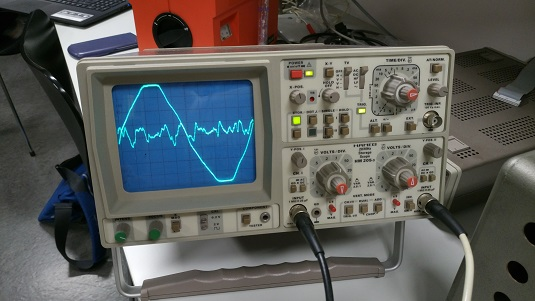
\includegraphics[scale=0.5]{Oszi.jpg}
  \caption{Oszilloskop mit Wechselstromsignal und Detektorsignal}
  \label{oszi}
\end{figure}

Um unsere Messungen vergleichen zu können, ist es wichtig diese bei gleichem Magnetfeld durchzuführen. Um die entsprechenden Resonanzfrequenzen bestimmen zu können, verändern wir die Frequenz des eingestrahlten Feldes kontinuierlich, bis sich die beiden am Oszilloskop erkennbaren Maxima genau aufheben. Dies geschieht genau am Maximum bzw. Minimum des magnetischen Wechselfeldes, sodass wir so den minimalen bzw. maximalen Wert des angelegten Magnetfelds bestimmen und annehmen können. Leider zeigen die verwendete Elektronik und Leitungen ein sehr hohes Rauschen, sodass die tatsächlichen Maxima im Detektorsignal nur sehr schwer vom Hintergrundrauschen zu unterscheiden waren. Aus diesem Grund nehmen wir für jede Messung 10 Messwerte am Magnetfeld-Maximum und -Minimum auf, um eventuelle Ungenauigkeiten herausmitteln zu können. 

Die aufgenommen Messwerte zusammen mit den berechneten Mittelwerten für die Resonanzfrequenzen finden sich in Tabelle \ref{freqs}.

\begin{table}[h]
	\caption{Resonanzfrequenzen der untersuchten Verbindungen}
	\begin{tabular}{|c|c|c|c|c|c|c|}
	\hline
	& \multicolumn{2}{|c|}{Glycerin} & \multicolumn{2}{|c|}{$CuSO_4$} & \multicolumn{2}{|c|}{Teflon} \\ \hline
	 & $f_{max}$ in kHz & $f_{min}$ in kHz & $f_{max}$ in kHz & $f_{min}$ in kHz & $f_{max}$ in kHz & $f_{min}$ in kHz\\ \hline
	 1 & 32415 & 31644 & 32409 & 31645 & 30486 & 29772 \\ \hline
	 2 & 32413 & 31648 & 32416 & 31642 & 30480 & 29781 \\ \hline
	 3 & 32408 & 31645 & 32410 & 31643 & 30480 & 29784 \\ \hline
	 4 & 32410 & 31649 & 32410 & 31645 & 30477 & 29788 \\ \hline
	 5 & 32416 & 31647 & 32409 & 31644 & 30469 & 29789 \\ \hline
	 6 & 32411 & 31648 & 32406 & 31646 & 30472 & 29780 \\ \hline
	 7 & 32411 & 31648 & 32408 & 31647 & 30479 & 29794 \\ \hline
	 8 & 32412 & 31645 & 32406 & 31647 & 30475 & 29782 \\ \hline
	 9 & 32410 & 31649 & 32408 & 31649 & 30477 & 29786 \\ \hline
	 10 & 32413 & 31647 & 32408 & 31647 & 30478 & 29789 \\ \hline \\ \hline
	 $ \varnothing $ & 32411,9 & 31647 & 32409 & 31645,5 & 30477,3 & 29784,5 \\ \hline
	 $\sigma$ & 2,3 & 1,7 & 2,7 & 2,0 & 4,4 & 5,8 \\ \hline
	\end{tabular}
\label{freqs}
\end{table}

Aus den aufgenommenen Werten für Glycerin können wir nun das angelegte Magnetfeld im Maximum und im Minimum berechnen. Dies ergibt sich zu:

\begin{gather}
B=\frac{f \cdot 2\pi}{\gamma} \\
B_{max}=\frac{32411,9 \cdot 10^3 \cdot 2\pi}{26,75 \cdot 10^7} \pm \frac{2,3 \cdot 10^3 \cdot 2\pi}{26,75 \cdot 10^7}  \approx 0,76131  \pm 0,00005 T \\
B_{min}=\frac{31647 \cdot 10^3 \cdot 2\pi}{26,75 \cdot 10^7} \pm \frac{1,7 \cdot 10^3 \cdot 2\pi}{26,75 \cdot 10^7}   \approx 0,74334 \pm 0,00004 T
\end{gather}

Mit diesen Werten und den gemessenen Resonanzfrequenzen können wir nun $\gamma$ und die g-Faktoren für $CuSO_4$ und Teflon bestimmen. 

\begin{table}[h]
	\caption{Experimentell bestimmte Faktoren}
	\begin{tabular}{|c|c|c|c|c|c|c|}
	\hline
	& \multicolumn{3}{|c|}{$CuSO_4$} & \multicolumn{3}{|c|}{Teflon} \\ \hline
	& $f_{max}$ & $f_{min}$  & $\varnothing $  & $f_{max}$ & $f_{min}$ &  $\varnothing$ \\ \hline
	Landé-Faktor g & 5,5855 & 5,5857 & 5,5856 & 5,2526 & 5,2572 & 5,2549 \\ \hline
	$\gamma \cdot 10^{-7}$ in rad. $T^{-1} s^{-1}$& 26,747 & 26,749 & 26,748 & 25,153 & 25,176 & 25,165 \\ \hline
	\end{tabular}
\label{gammas}
\end{table}	


